\documentclass[11pt]{article}
\usepackage[margin=1in]{geometry}
\usepackage{natbib}
\usepackage{amsmath,amssymb,amsthm,bm,xcolor,hyperref,booktabs,enumitem,graphicx}
\theoremstyle{plain}\newtheorem{theorem}{Theorem}\newtheorem{lemma}{Lemma}\newtheorem{proposition}{Proposition}
\theoremstyle{definition}\newtheorem{assumption}{Assumption}\newtheorem{remark}{Remark}
\newcommand{\E}{\mathbb{E}}\newcommand{\R}{\mathbb{R}}\newcommand{\N}{\mathcal{N}}\newcommand{\corr}{\mathrm{corr}}
\newcommand{\GP}{\mathcal{GP}}
\hypersetup{colorlinks=true,allcolors=blue!55!black}

\title{\textbf{Structure as Covariance: When a Graph Kernel Helps\\ Budget-Limited Active Retrieval}}
\author{Robert Richardson}
\date{\today}

\begin{document}\maketitle

\begin{abstract}
In multi-hop retrieval-augmented generation, relevance judgments are expensive LLM calls, so retrieval under a
judgment budget is a problem of Bayesian experimental design. We show that the corpus graph---which does
\emph{not} help as a ranking signal, because diffusion buries the answer---becomes load-bearing as the
\emph{covariance} of a latent relevance field with a semantic (retriever) mean: a judgment of one candidate
propagates belief to graph-connected candidates, surfacing a buried ``bridge'' passage that no single embedding
neighbour reveals. We make three contributions. \emph{(i)} A model---a Gaussian process with a semantic mean and a
graph covariance---together with the initially surprising finding that the graph kernel must be used in
\emph{correlation} (unit-diagonal) form, which roughly doubles its effect by equalizing hub variance so that
optimistic exploration reaches the propagating anchors. \emph{(ii)} An \emph{alignment law}: we prove, under a
stochastic block model, that the structural gain is zero when the graph is unaligned with the reasoning chain,
positive iff the graph is chain-\emph{assortative}, and monotone in a scalar alignment $p-q$ estimated in practice
by the empirical \emph{assortativity} $\hat p-\hat q$; the oracle-graph ceiling and the failure on adversarial
corpora are the two ends of this one axis. The same analysis gives a \emph{mechanism} for why optimistic
exploration suits this problem---the value of a judgment is the downstream surfacing it enables, a delayed quantity
that one-step value-of-information undervalues---while the full superiority of UCB over multi-step lookahead we
report as an empirical finding rather than a theorem. \emph{(iii)} An empirical characterization under a real
hop-aware judge across HotpotQA, 2WikiMultiHopQA, and MuSiQue: a significant low-budget win on standard multi-hop
(recall $+0.058$, nDCG@10 $+0.030$, chain-completion $+0.122$ at one judgment) that holds head-to-head against a
faithful re-implementation of BAGEL at matched budget---where the covariance advantage is \emph{budget-invariant}
(a constant $\approx+0.11$ recall@$k$ from $B{=}1$ to BAGEL's native $B{=}50$, controlling for the prior), hence not
a low-budget artifact---and $\approx+0.15$ at a $5\times$ deeper $N{=}500$ pool, so not a small-pool one either---while BAGEL's embedding kernel plateaus $\sim0.12$ below ours even at its own native
budget---a partial rescue of
adversarial MuSiQue by
inferring the graph from the judge's own hop-reasoning ($+0.035$ at three hops, where every cheap surface graph is
null), and an honest analysis of why the natural
adaptive gate does \emph{not} deploy---the per-query gain is a small distributional effect (signal-to-noise
$\approx 0.1$--$0.2$) rather than a per-query-predictable signal, so using the graph across the multi-hop regime
it targets is the correct, simple policy. Effects are modest but principled.
\end{abstract}

\section{Introduction}
Retrieval-augmented generation increasingly relies on an LLM to \emph{judge} candidate passages, at a real
per-call cost. When the budget is a handful of judgments per query, retrieval becomes active learning: which
candidates should we spend judgments on, and how should a judgment reshape our beliefs about the rest? The hard
case is multi-hop: a question whose answer requires chaining facts across passages, where one gold passage---the
\emph{bridge}, supplying a linking entity rather than the answer itself---has low retriever similarity to the
query and sits buried among distractors. A bridge is exactly what an embedding retriever misses and what a
dependency structure could recover, if a judgment on a findable passage could \emph{propagate} to it.

\paragraph{Thesis: semantics sets the mean, structure sets the dependence.} We model latent relevance as a
Gaussian process whose \emph{mean} is a calibrated retriever score and whose \emph{covariance} is a corpus graph.
The graph is a poor ranking signal---using it to re-score \emph{buries} the bridge under diffusion---but an
excellent covariance: ``connected passages have correlated relevance,'' so conditioning on a judged anchor lifts
the posterior mean of a connected bridge. The same object that hurts as a mean helps as a dependence. This
resolves a tension in graph-based retrieval and, we argue, is the reason a Bayesian treatment earns its keep here:
the graph enters the \emph{decision/experimental-design} layer, not the ranking layer.

\paragraph{Contributions.}
\begin{enumerate}[leftmargin=*,itemsep=1pt,topsep=2pt]
\item \textbf{Model + the normalization finding} (\S\ref{sec:model}): a GP with a semantic mean and a graph
covariance, and the finding that the graph kernel must be in correlation (unit-diagonal) form---which
$1.8\times$s its effect (chain-completion margin $+0.068\to+0.122$) by equalizing hub variance so optimistic
exploration reaches the propagating anchors.
\item \textbf{The alignment law} (\S\ref{sec:law}): a surfacing lemma and a stochastic-block-model theorem---the
structural gain is $0$ at zero alignment, positive iff the graph is chain-assortative ($p>q$), and monotone in
$p-q$; the oracle ceiling and the adversarial failure are the two ends of one axis, measured by the empirical
assortativity $\hat p-\hat q$. The same surfacing analysis gives a mechanism for why optimistic acquisition suits
this problem, though the full superiority of UCB over multi-step lookahead we leave as an empirical finding
(\S\ref{sec:acq}).
\item \textbf{An honest empirical characterization} (\S\ref{sec:exp}) under a real hop-aware judge: a significant
low-budget win on standard multi-hop that survives a head-to-head with a faithful BAGEL re-implementation; a
partial rescue of adversarial MuSiQue via an LLM hop-assignment graph; and
an analysis of why per-query adaptive routing does not deploy, so that within the deep multi-hop regime studied a
global graph policy is better supported than per-query routing.
\end{enumerate}
We do not claim large gains: effects are modest. We claim a principled account---\emph{when} structure helps and
\emph{why}---and a method that did not significantly hurt in the regimes we tested, and is simple.

\section{Related work}\label{sec:rel}
\emph{Active / Bayesian retrieval.} Our nearest neighbour is BAGEL~\citep{bagel2026}, a query-specific GP-UCB over
passage embeddings; our data refute the embedding kernel here and replace it with a graph covariance, and we add a
soft (noisy-likelihood) update that prevents a GP from confidently propagating a wrong LLM label---BAGEL's two named
limitations. We compare against a faithful re-implementation head-to-head (\S\ref{sec:exp}, Figure~\ref{fig:bagel}). \emph{Graph retrieval.} GraphRAG and HopRAG use graph structure for retrieval; HopRAG builds logical
pseudo-query edges precisely because surface similarity is insufficient, consonant with our alignment law. We use
the graph as a covariance, not a ranking signal, and characterize when it helps. \emph{GMRF/CAR priors} (Rue \&
Held) supply the kernel; \emph{Bayesian optimization / value of information} the acquisition; \emph{set-wise
retrieval} (SETR) the completion metric. Our novelty is the mean/dependence decomposition, the exploration
mechanism, and the alignment regime---not any single primitive.

\section{Model: structure as covariance}\label{sec:model}
Per query, a first-stage retriever returns $N$ candidates with normalized embeddings $v_i$ and retriever scores;
a calibrated logistic map gives a prior mean $m_i\in[0,1]$ (cross-fit cosine$\to$gold). We place a GP on latent
relevance $f\sim\GP(m,K)$ and, when candidate $j$ is judged, observe $y_j\in\{0,\tfrac12,1\}$ (a graded hop-aware
label) under Gaussian noise $\sigma^2$. Ranking is by posterior mean; recall@$k$, chain-completion, and nDCG@10
are measured against gold.

\paragraph{Two kernels.} The embedding kernel $K^E_{ij}=\exp(-(1-v_i^\top v_j)/\ell)$ encodes ``similar
embeddings, similar relevance''---but the bridge is dissimilar to everything, so $K^E$ cannot reach it. The graph
kernel is a GMRF/CAR covariance $K^G=(I+\lambda \mathcal L)^{-1}$ on a corpus graph $A$ (Laplacian
$\mathcal L=D-A$), encoding ``connected passages, correlated relevance.''

\paragraph{The load-bearing detail: correlation form.} We find the graph kernel must be normalized to unit
diagonal, $\widetilde K^G=\mathrm{diag}(K^G)^{-1/2}K^G\,\mathrm{diag}(K^G)^{-1/2}$, before use. Unnormalized, high-degree
hubs have \emph{lower} prior variance, so an upper-confidence-bound rule under-explores them---but the hubs are
exactly the anchors whose judgment propagates to bridges. Equalizing variance lets exploration reach the hubs; the
propagation then fires. Empirically this $1.8\times$ the graph$-$cosine chain-completion margin ($+0.068\to+0.122$
at one judgment) and, unlike the raw kernel (which converges to null by three judgments), keeps the win
significant at every budget. The finding is a small but real methodological point and is, to our knowledge, not
standard in GP-active-retrieval practice.

\paragraph{The soft update.} Conditioning on judged set $J$, $\mu = m + K_{:J}(K_{JJ}+\sigma^2 I)^{-1}(y_J-m_J)$.
We rank by $\mu$ (soft) rather than hard-pinning judged labels; with an imperfect judge, hard pinning of a wrong
label is catastrophic (a mislabeled gold is sunk), while the soft update degrades gracefully.

\section{Acquisition: exploration, not information}\label{sec:acq}
We select judgments by UCB, $\arg\max_i \mu_i+\beta\,\mathrm{sd}_i$. Against principled alternatives---one-step
value of information for chain completion ($1-\prod_j(1-p_j)$), two-step lookahead, pure information gain (maximum
variance reduction), and pure exploration (maximum variance)---UCB wins across the board on the graph kernel
(chain-completion $-0.08$ to $-0.11$ at one judgment; two-step lookahead does not help either). We separate the
mechanism from the empirical finding. \emph{Mechanism:} the value of judging a high-prior anchor is not its own
label but the \emph{downstream} surfacing of a connected bridge (Lemma~\ref{lem:surface})---a delayed value that a
myopic one-step completion objective structurally undervalues, which explains why one-step VOI loses. \emph{Open:}
this does \emph{not} obviously explain why our two-step lookahead and information gain also lose---a faithful
short-horizon policy should see the delayed value---so \emph{why optimism remains superior to short-horizon
lookahead here is an empirical finding we do not fully explain.} What UCB does that the others miss is focus
exploration, via its mean term, on the high-prior anchors along which belief propagates; kernel and acquisition
are entangled, and the graph \emph{needs} UCB. (Theorem~\ref{thm:align} is a surfacing result conditional on
judging the anchor; it is not itself an acquisition-optimality theorem.)

\section{The alignment law}\label{sec:law}
When does the graph help? We give an exact surfacing condition and lift it to a statistical law.
\begin{assumption}[Buried bridge]\label{ass:bridge}
Gold $=\{a,b\}$ with $m_a=\max_i m_i$ (findable anchor) and $m_b<\min_{d}m_d$ (bridge buried below distractors
$D$); judging is informative, $y_a>m_a$.
\end{assumption}
\begin{lemma}[Surfacing]\label{lem:surface}
With unit prior variances the first UCB pick is $a$; conditioning gives $\mu_i=m_i+\frac{K_{ia}}{1+\sigma^2}
(y_a-m_a)$, and the bridge enters the top-$k$ iff the \emph{kernel differential} exceeds the burial threshold,
\[
   K_{ba}-\max_{d\in D}K_{da}\ >\ \tau:=\frac{(1+\sigma^2)(\max_d m_d-m_b)}{y_a-m_a}.
\]
\end{lemma}
The mechanism is isolated: a judgment surfaces the bridge only through a kernel that couples it to the findable
anchor \emph{more} than it couples distractors. The embedding kernel has this differential $\le 0$ for a buried
bridge, so it never surfaces it; the graph kernel can.

\begin{theorem}[Alignment law]\label{thm:align}
Let the graph be a stochastic block model with within-chain edge probability $p$, off-chain $q$ (alignment
$p-q$). \emph{(i) One-hop, exact.} For the one-hop kernel $\corr(I+\beta A)$ with $0<\tau<\beta$, the bridge
surfaces iff $A_{ba}=1$ and $A_{da}=0\ \forall d$, so $\Pr(\text{surface})=p(1-q)^{|D|}$; the \emph{alignment
excess} over a density-matched unaligned graph (chain edge also at rate $q$) is
\[
   \Delta_{\mathrm{align}}(p,q)=\Pr_{p,q}(\text{surface})-\Pr_{q,q}(\text{surface})=(p-q)\,(1-q)^{|D|},
\]
which is $0$ at $p=q$, positive iff $p>q$, and (fixed $q$) exactly linear in $p-q$. \emph{(ii) Actual GMRF, first
order.} The method's kernel $\corr\big((I+\lambda L)^{-1}\big)$ has $\E[K_{ba}-K_{da}]=\lambda(p-q)+O(\lambda^2)$.
\emph{(iii) Limits.} $q\to0,p\to1$ (gold clique) maximizes the excess; $p\approx q$ (edges independent of the
chain---surface-similar distractors) gives $\Delta_{\mathrm{align}}\approx0$.
\end{theorem}
Proof in Appendix~\ref{app:proof}. Note the excess, not the raw surfacing probability, is what vanishes at $p=q$:
an unaligned graph surfaces the bridge with probability $q(1-q)^{|D|}>0$ by chance, so the empirical gain at $p=q$
is small but nonzero (Figure~\ref{fig:align}A); the alignment law governs the \emph{excess}. We verify all parts
in \texttt{paperA\_alignment\_sim.py}: the one-hop rate matches $p(1-q)^{|D|}$, the excess matches
$(p-q)(1-q)^{|D|}$, and the GMRF differential is $\propto p-q$. The real data (Figure~\ref{fig:align}B) trace the
same law against empirical assortativity, from aligned (chained) through neutral (comparison) to the adversarial
MuSiQue boundary.
\begin{figure}[t]\centering
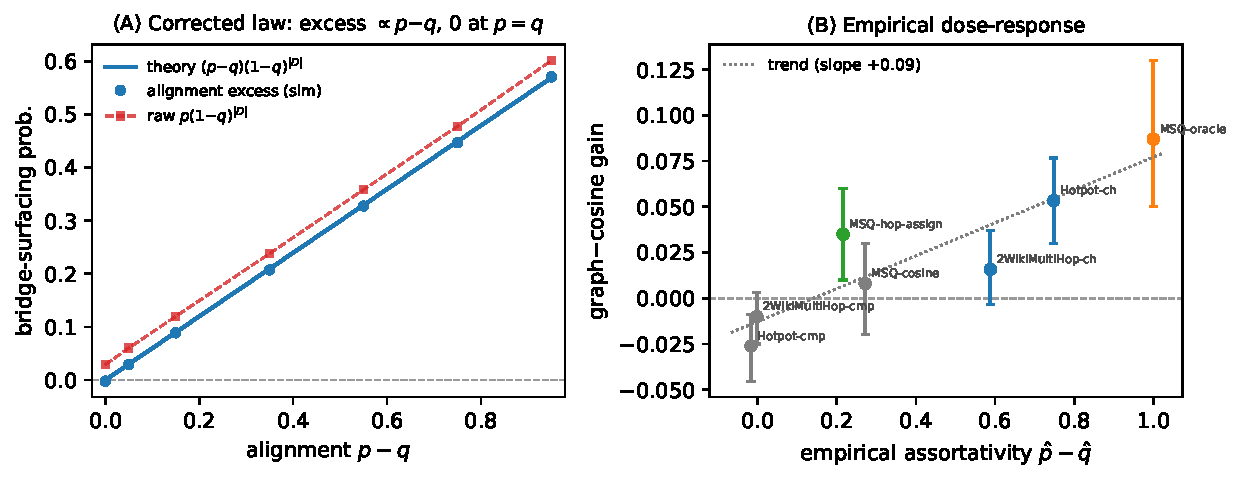
\includegraphics[width=\linewidth]{fig_alignment.pdf}
\caption{The alignment law. \textbf{(A)} The alignment excess $(p-q)(1-q)^{|D|}$ vanishes at $p=q$ and is linear in
$p-q$ (theory line and one-hop simulation), while the \emph{raw} surfacing probability $p(1-q)^{|D|}$ stays
positive---an unaligned graph surfaces the bridge by chance, so the law governs the \emph{excess}, not the raw
probability. \textbf{(B)} Empirical dose-response: real graph$-$cosine recall gain vs.\ empirical graph--chain
assortativity $\hat p-\hat q$ across datasets and graph constructions---comparison ($\approx0$ assortativity,
$\approx0$ gain), chained (high, positive), adversarial-MuSiQue cheap graphs (null) up to the oracle clique (max);
the LLM hop-assignment graph slightly exceeds its global assortativity (better-placed edges). Bars are $95\%$ CIs.}
\label{fig:align}
\end{figure}
\begin{remark}[Measurable alignment]
In practice $p-q$ is estimated by the empirical graph--chain \emph{assortativity} $\widehat A=\hat p-\hat q$ (the
gold--gold edge rate minus the gold--distractor edge rate); gold-connectivity alone estimates $\hat p$ only.
Theorem~\ref{thm:align} explains why $\widehat A$ predicts the gain, why the oracle ceiling and the adversarial
failure are one axis, and why the effect saturates.
\end{remark}

\section{Experiments}\label{sec:exp}
\paragraph{Setup.} Pools of $N=100$ retrieved from a full-dev corpus (so the bridge is genuinely buried and the
prior is weak); a graded $0$--$2$ hop-aware LLM judge (gpt-4o-mini) that explicitly credits linking passages; the
soft GP with $\sigma^2$ tuned to judge reliability. Baselines: no-judge prior, passive verify-top-$B$,
embedding-kernel GP, a faithful re-implementation of BAGEL~\citep{bagel2026}, and ceilings (oracle judge, oracle
graph). Metrics: recall@$k$, chain-completion
($k=|\text{gold}|$), nDCG@10; paired bootstrap 95\% CIs; query-grouped splits. Datasets: HotpotQA,
2WikiMultiHopQA, MuSiQue. A naive judge (``does this answer the question?'') is bridge-blind (gold recall $0.35$);
the hop-aware prompt raises gold recall to $0.84$, isolating the prompt fix from model strength.

\paragraph{Main result: a significant low-budget win on standard multi-hop.} On chained HotpotQA/2Wiki
($n{=}600$), with the correlation-form kernel the graph beats the embedding kernel across all three metrics and all
budgets (Table~\ref{tab:main}): at one judgment, recall $+0.058\,[.040,.076]$, nDCG@10 $+0.030\,[.020,.041]$,
chain-completion $+0.122\,[.088,.155]$; significant through $B{=}3$. The graph kernel---not ``any GP''---drives it:
graph-GP $>$ cosine-GP $>$ passive. The win is individually significant in \emph{each} corpus, larger on the more
assortative one (HotpotQA $>$ 2Wiki; Appendix~\ref{app:perds}).
\begin{table}[t]\centering\small
\begin{tabular}{lccc}
\toprule
graph$-$cosine (chained, real judge) & recall@$k$ & nDCG@10 & completion \\ \midrule
$B=1$ & $+0.058\,[.040,.076]$ & $+0.030\,[.020,.041]$ & $+0.122\,[.088,.155]$ \\
$B=2$ & $+0.071\,[.052,.090]$ & $+0.032\,[.021,.045]$ & $+0.150\,[.115,.185]$ \\
$B=3$ & $+0.063\,[.044,.082]$ & $+0.033\,[.022,.045]$ & $+0.127\,[.093,.162]$ \\
\bottomrule
\end{tabular}
\caption{Low-budget graph-kernel win (correlation-form kernel), significant at all budgets. The raw kernel is
weaker and converges to null by $B=3$ (\S\ref{sec:model}, normalization).}\label{tab:main}
\end{table}

\paragraph{Is the graph just a proxy the embedding covariance could supply? No: the mixture picks pure graph.}
A natural worry is that we discard useful embedding covariance. We test the fixed convex family
$K_\alpha=(1-\alpha)\widetilde K^E+\alpha\widetilde K^G$ (both correlation-form, \emph{same} calibrated mean),
sweeping a single global $\alpha$ on the chained set. Recall@$k$ rises \emph{monotonically} in the graph weight,
$0.634\ (\alpha{=}0,\text{embedding covariance})\to0.692\ (\alpha{=}1,\text{graph})$ at $B{=}1$, and completion
$0.323\to0.445$; the tuned optimum is $\alpha^\star=1$. Holding the mean fixed and varying only the covariance, the
graph is the better covariance and the embedding covariance adds nothing on top of it---a dose-response in the
mixing weight that mirrors the alignment dose-response, and a direct answer to ``why not keep the embedding
covariance.''

\paragraph{Head-to-head with the actual BAGEL algorithm, across the full budget range.} Our nearest competitor is
BAGEL~\citep{bagel2026}. We reimplement it faithfully (code unreleased): a query-specific \emph{zero-mean} GP over
passage embeddings with an RBF kernel whose lengthscale is fit \emph{per query} by marginal likelihood, LLM
relevance scores as standardized observed labels, the query embedding seeded as a maximum-relevance
pseudo-observation, a top-$M$ dense warm-start, UCB acquisition ($\beta{=}2$), and final ranking by posterior mean;
we match its total judgment budget to ours and sweep $B$ from $1$ to $50$---up to and including BAGEL's \emph{exact
native configuration} ($B{=}50=25$ warm-start $+\,25$ active judgments, half the $N{=}100$ pool). The graph method
beats faithful BAGEL on recall@$k$ at every budget (Figure~\ref{fig:bagel}A), and---this is the load-bearing
fairness check---the gap decomposes into a budget-\emph{sensitive} mean effect and a budget-\emph{invariant}
covariance effect (Figure~\ref{fig:bagel}B). \emph{(i) Semantics-in-the-mean:} BAGEL's zero-mean GP carries no
cross-query prior and is starved when the budget is tiny; giving BAGEL's own kernel our calibrated prior mean
(``$+$our prior'') recovers this part, and it is the \emph{only} part that shrinks with budget ($\Delta$ falls from
$+0.25$ at $B{=}1$ toward $+0.12$). \emph{(ii) Structure-in-the-covariance:} even with our prior \emph{and} BAGEL's
marginal-likelihood-tuned RBF kernel and query-seed, the graph covariance wins by a \emph{constant} $\approx +0.11$
recall@$k$ from $B{=}1$ all the way to BAGEL's native $B{=}50$ ($+0.109,\dots,+0.114,+0.114$)---so the covariance
advantage is \emph{not} a low-budget artifact, and BAGEL's kernel-tuning does not close it at any budget. Indeed
faithful BAGEL \emph{plateaus} at recall $\approx 0.58$ from $B{=}10$ on, $\sim0.12$ below ours even at its own
native budget: its embedding covariance structurally cannot surface a bridge that is semantically far from the
anchor, so more judgments do not rescue it.

\emph{(iii) Not a small-pool artifact.} Re-running the head-to-head at a $5\times$ deeper pool ($N{=}500$, so
budgets $B{=}1$--$50$ probe only $0.2$--$10\%$ of the candidates---the regime a deployed system actually
faces) leaves the covariance gap flat across budget and \emph{larger}: $\approx+0.15$ recall@$k$
($+0.142,\dots,+0.189$ over $B{=}1$--$50$, every interval excluding zero and above its $N{=}100$ value;
Figure~\ref{fig:bagel}B). The mechanism is the one that makes structure load-bearing here: a deeper pool
buries the bridge further, exactly where the embedding covariance fails and the graph covariance pays off, so
graph-GP recall stays pool-robust ($0.67$--$0.72$) while faithful BAGEL degrades ($0.39$--$0.56$). The
covariance advantage is thus neither a low-budget nor a small-pool artifact.
The conclusion is unchanged under a maximally-active warm/active split (warm$=1$: $\Delta$ vs BAGEL $+0.24$, vs
$+$prior $+0.13$ at $B{=}3,5$).
\begin{figure}[t]\centering
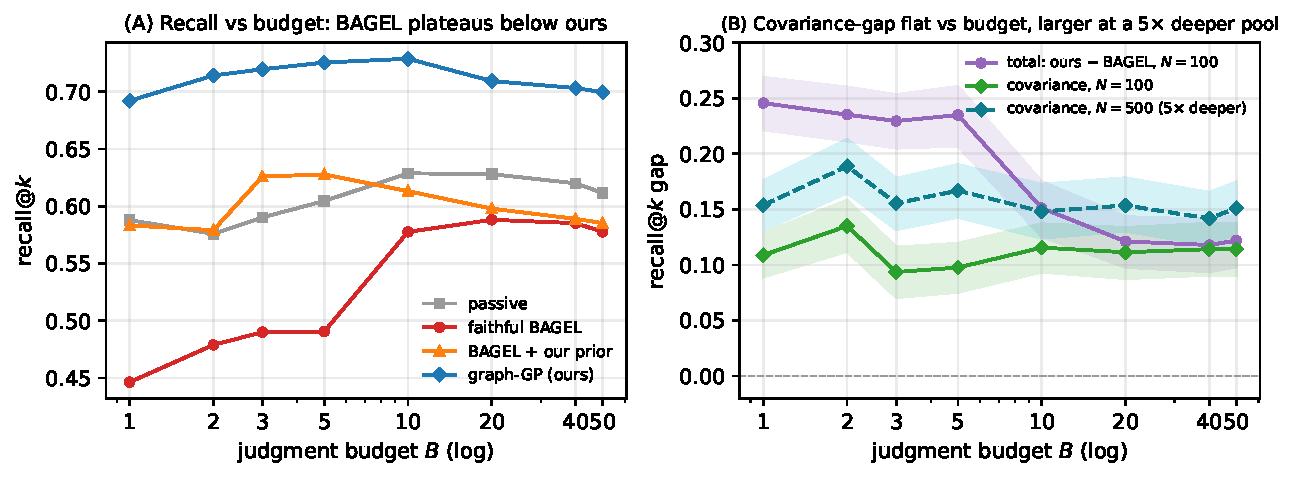
\includegraphics[width=\linewidth]{fig_bagel.pdf}
\caption{Faithful BAGEL vs.\ ours at matched judgment budget (chained, $n{=}600$; $B$ up to BAGEL's native $50$).
\textbf{(A)} BAGEL plateaus $\sim0.12$ recall@$k$ below ours even at its native budget. \textbf{(B)} The total gap (ours$-$BAGEL) shrinks as
BAGEL's zero-mean starvation eases, but the covariance gap (ours$-$(BAGEL$+$our prior), same mean) is
budget-invariant: $\approx+0.11$ at $N{=}100$, and at a $5\times$ deeper $N{=}500$ pool flat and \emph{larger} at $\approx+0.15$ (bands are 95\% CIs). The graph advantage is neither a low-budget nor a small-pool artifact.}
\label{fig:bagel}
\end{figure}

\paragraph{The alignment law, from both sides.} We judged the \emph{comparison} (independent-evidence) questions
as a control, giving a mixed distribution ($300$ chained $+$ $300$ comparison). The graph helps chained
($+0.058\,[.040,.076]$ at $B{=}1$) and does \emph{not} help comparison (neutral to slightly negative,
$\le 0$)---the boundary the theorem predicts, with the mechanism visible: comparison questions have a strong prior
(passive recall $\sim0.8$; both entities directly findable, no bridge to propagate along). The oracle-graph
ceiling is $+0.07$--$0.09$, and the empirical assortativity $\hat p-\hat q$ tracks the per-regime gain
(Figure~\ref{fig:align}B).

\paragraph{Adversarial corpora: MuSiQue, and a partial rescue.} MuSiQue's distractors are made surface-similar to
golds, so cheap graphs (title, entity-overlap, cosine-decomposition) have $p\approx q$ and are null
(graph$-$cosine $+0.008\,[\text{-}.02,.03]$ at three hops), while an oracle gold-clique graph recovers
$+0.087\,[.05,.13]$---exactly the theorem's two ends. Following its prescription (raise $p-q$), we build the graph
from the judge's \emph{own} reasoning: decompose the question into sub-questions and ask the judge which
sub-question each pool passage answers, then connect passages on different hops. This recovers a significant
$+0.035\,[.01,.06]$ at three hops---$\sim4\times$ the cosine graph and $\sim40\%$ of the oracle headroom, robust
across graph constructions---where every surface graph is null. \emph{Budget accounting (important).} These
hop-assignments are \emph{extra} LLM calls over the pool, outside the judgment budget $B$ that the retrieval
methods share; we therefore report this as a \emph{structure-construction} experiment---evidence that a
chain-assortative graph, once built, recovers the covariance gain the oracle predicts---\emph{not} as a
budget-fair competitor. The budget-fair version is to elicit the hop/role assignment in the \emph{same} call as
the relevance grade (one call per judged node returns \emph{(grade, role)}), turning graph construction into a
by-product of the existing budget; realizing that adaptive ``judge $\to$ learn relevance $+$ role $\to$ update
graph $\to$ choose next'' loop is the natural sequel. As reported, it is a proof-of-concept that inferring
structure from the judge's reasoning is the route to adversarial corpora.

\paragraph{Why not adapt per query? An honest negative.} A natural extension is a gold-free gate that decides
per query whether to use the graph. It does not deploy, and the reason is instructive and robust to the kernel
choice. The per-query graph advantage is a \emph{small mean effect swamped by variance} (signal-to-noise
$\approx0.1$--$0.2$) and is nearly unpredictable from gold-free features \emph{even under the oracle}: ridge
$R^2\approx0.03$--$0.05$, and only marginally better with theory-motivated alignment/reachability features. Two
mechanistic fixes we tried failed: the graph does \emph{not} amplify judge errors (advantage correlates $-0.17$
with anchor reliability), and confidence-gating the propagation to high-confidence labels \emph{hurts} ($-0.030$;
the ``related'' grade-$1$ labels carry useful signal). On the mixed distribution the learned gate only \emph{ties}
always-graph ($+0.003$, n.s.) while the per-query oracle has a real $+0.027$ headroom that is simply not
gold-free-reachable---and this holds under the correlation-form kernel, even though there the graph slightly
\emph{penalizes} comparison queries. The structural gain is thus a \emph{distributional} property---a robust
average in the deep multi-hop regime (the alignment law)---not a per-query-predictable signal. The correct policy
is to use the graph in the multi-hop regime it targets; per-query adaptivity is neither feasible nor needed.

\section{Discussion and limitations}\label{sec:disc}
Effects are modest and low-budget; the BAGEL comparison is a faithful re-implementation (their code is unreleased),
though we control for its prior and lengthscale-fitting so the covariance advantage is not an implementation
artifact; two of three benchmarks are standard multi-hop. The contribution is the account: a mean/dependence decomposition, a proved alignment law that unifies
the oracle ceiling and the adversarial boundary, an exploration mechanism, and an honest map of where the method
helps (deep multi-hop with a chain-assortative graph), is neutral (independent evidence), and is only partially
recoverable (adversarial corpora, via inferred structure). The deepest open direction is \emph{adaptive structure
learning}: inferring the reasoning-chain graph from the first judgments---of which the MuSiQue hop-assignment
result is a first instance---which would raise $p-q$ within the budget and is the most plausible route to helping
on adversarial corpora without a gold-derived graph.

\appendix
\section{Proof of Theorem~\ref{thm:align}}\label{app:proof}
\emph{(i)} The one-hop kernel has $K_{ij}=\beta A_{ij}$ for $i\neq j$, so by Lemma~\ref{lem:surface} surfacing
requires $\beta(A_{ba}-\max_d A_{da})>\tau$; since $A\in\{0,1\}$ and $0<\tau<\beta$, this holds iff $A_{ba}=1$ and
$\max_d A_{da}=0$. Independence of the edges gives $\Pr(\text{surface})=\Pr(A_{ba}=1)\prod_d\Pr(A_{da}=0)=
p(1-q)^{|D|}$. The density-matched unaligned graph replaces $p$ by $q$, giving $q(1-q)^{|D|}$; subtracting yields
$\Delta_{\mathrm{align}}=(p-q)(1-q)^{|D|}$, which is $0$ at $p=q$, positive iff $p>q$, and linear in $p-q$ at fixed
$q$. \emph{(ii)} $(I+\lambda L)^{-1}=I-\lambda L+O(\lambda^2)$ with $L=D-A$, so the off-diagonal is
$K_{ij}=\lambda A_{ij}+O(\lambda^2)$; correlation normalization divides by $\sqrt{K_{ii}K_{jj}}=1+O(\lambda)$ and
preserves the first-order term, whence $\E[K_{ba}-K_{da}]=\lambda(p-q)+O(\lambda^2)$. \emph{(iii)} Immediate from
$\Delta_{\mathrm{align}}=(p-q)(1-q)^{|D|}$: maximal at $q{=}0,p{=}1$, zero at $p=q$. \hfill$\square$

\section{Per-dataset breakdown}\label{app:perds}
The pooled headline (Table~\ref{tab:main}) is significant in \emph{each} dataset separately, so pooling is not
masking a null (Table~\ref{tab:perds}). HotpotQA, whose chained graph is more chain-assortative
($\hat p-\hat q=0.75$ vs.\ $0.59$ for 2Wiki), shows the larger gain at every budget and metric---the same
dose-response ordering as Figure~\ref{fig:align}B, now \emph{across} standard corpora rather than within one.
\begin{table}[h]\centering\small
\begin{tabular}{llccc}
\toprule
$B$ & dataset ($n{=}300$) & recall@$k$ & nDCG@10 & completion \\ \midrule
$1$ & HotpotQA & $+0.073\,[.048,.098]$ & $+0.041\,[.026,.055]$ & $+0.153\,[.103,.203]$ \\
$1$ & 2Wiki    & $+0.043\,[.020,.068]$ & $+0.020\,[.005,.035]$ & $+0.090\,[.047,.137]$ \\
$2$ & HotpotQA & $+0.090\,[.063,.118]$ & $+0.040\,[.025,.056]$ & $+0.180\,[.130,.233]$ \\
$2$ & 2Wiki    & $+0.051\,[.028,.077]$ & $+0.025\,[.008,.041]$ & $+0.120\,[.077,.167]$ \\
\bottomrule
\end{tabular}
\caption{Graph$-$cosine margin per dataset (correlation-form kernel, pooled calibration). Both are individually
significant at $B{=}1,2$; the more assortative corpus (HotpotQA) gains more.}\label{tab:perds}
\end{table}

\smallskip\noindent\footnotesize\emph{Reproducibility.} All experiments use cached judgments; scripts and the full
experimental log accompany the submission. Total LLM spend for all runs reported here is under \$10.

\normalsize
\begin{thebibliography}{1}
\bibitem[Kim et al.(2026)]{bagel2026} J.~Kim, A.~Korikov, J.~Liang, J.~Cui, Y.~S.~Liu, Q.~Wen, M.~Zhao, and
S.~Sanner. Bayesian active learning with Gaussian processes guided by {LLM} relevance scoring for dense passage
retrieval. \emph{arXiv preprint arXiv:2604.17906}, 2026.
\end{thebibliography}
\end{document}
